\scanpage{279}
\uline{Schémas polarisés}

Soit $X$ projectif sur $S$ loc. noeth., \inserted{plat et Steinien,}\deleted{\unsure{Noter qu'une} \uline{polarisation stricte} de $X$ est la donnée d'un élément de \deleted{$\unsure{\operatorname{Pic}(X/S)}$} $\operatorname{Pic}(X)$, \deleted{\illegible{1}}\inserted{\unsure{no.}} qui induit sur chaque fibre de $X/S$ un faisceau inversible \unsure{qui est} \illegible{2}}
\margin{semble excessif, par exemple pour l'énoncé du th. de Matsusaka}
\margin{\deleted{\unsure{défini par} \illegible{2} \unsure{inversible} \illegible{2} $X/S$}}

On suppose que $\uuline{\operatorname{Pic}}_{X/S}$ existe. Soit $\deleted{\unsure{\operatorname{Pol}}}\inserted{\operatorname{N\acute{e}r}}'(\unsure{X'|X}/S)$ l'ensemble quotient de $\operatorname{Pic}(X)^{\deleted{\unsure{X/S}}}$ \deleted{$\unsure{0}$} par $\operatorname{Pic}^{\deleted{\unsure{\tau}}}(X)^{\tau/S}$, où $\operatorname{Pic}(X)^{\tau/S}$ est l'image inverse de $\Gamma(S,\uuline{\operatorname{Pic}}^{\tau}_{X/S})$ par $\operatorname{Pic}(X)\to\Gamma(S,\uuline{\operatorname{Pic}}_{X/S})$. Les éléments de $\operatorname{N\acute{e}r}'(X/S)$ s'appellent \deleted{\unsure{pseudo}\uline{polarisations}}\inserted{\unsure{néronisations}} \uline{strictes}. On pose $\uline{\deleted{\unsure{\operatorname{Pol}}}\inserted{\operatorname{N\acute{e}r}}}'_{X/S}(T)=\deleted{\unsure{\operatorname{Pol}}}\inserted{\operatorname{N\acute{e}r}}'(X_T/T)$, c'est un foncteur contravariant en $T$, soit $\uline{\deleted{\unsure{\operatorname{Pol}}}\inserted{\operatorname{N\acute{e}r}}}'_{X/S}$, \deleted{multiplicatif} \unsure{donc} \illegible{1} \deleted{est} \unsure{au moins un préfaisceau}, $\rho$
\margin{$\rho$ et tel que pour $T'\to T$ fid plat de type fini, $\uline{\deleted{\unsure{\operatorname{Pol}}}\inserted{\operatorname{N\acute{e}r}}}'_{X/S}(T)\to\uline{\deleted{\unsure{\operatorname{Pol}}}\inserted{\operatorname{N\acute{e}r}}}'_{X/S}(T')$ soit injectif [i.e. les morphismes fid plats de type fini sont de descente pour $\uline{\operatorname{Pol}}'_{X/S}$]}

Rendons ce foncteur compatible avec la descente fid plate de type fini, on trouve un foncteur $\uline{\deleted{\unsure{\operatorname{Pol}}}\inserted{\operatorname{N\acute{e}r}}}^{\deleted{\unsure{\tau}}\prime\prime}_{X/S}$. \deleted{Un élément de} \unsure{On pose} $\uline{\deleted{\unsure{\operatorname{Pol}}}\inserted{\operatorname{N\acute{e}r}}}''_{X/S}(S)=\deleted{\unsure{\operatorname{Pol}}}\inserted{\operatorname{N\acute{e}r}}''(X/S)$, les éléments de cet ensemble s'appellent les \deleted{\unsure{pseudo}\uline{prépolarisations}}\inserted{\unsure{néronisations}} \uline{de $X$ sur $S$}. Donc :
\[
\text{(a)}\quad\uline{\deleted{\unsure{\operatorname{Pol}}}\inserted{\operatorname{N\acute{e}r}}}''_{X/S}(T)\simeq\deleted{\unsure{\operatorname{Pol}}}\inserted{\operatorname{N\acute{e}r}}''(X_T/T)\quad\text{(isom can)},
\]
une prépolarisation de $X/S$ est définie par la donnée d'une polarisation stricte $\xi$ d'un $X_T/T$,\inserted{i.e. d'un $\uline{L}$ inversible \deleted{\unsure{rel. ample}} sur $X_T/T$,} où $T$ est fid plt de type fini sur $S$, tel que les deux images inverses de $\xi$ sur $X_{T\times_S T}/T\times_S T$ soient identiques, i.e. tel $L$ \unsure{que} $p_1^*(\uline{L})p_2^*(\uline{L})^{-1}$ soit de \deleted{torsion}\inserted{\unsure{équiv. à $0$}} \unsure{rel.} à $T\times_S T$.
\figure{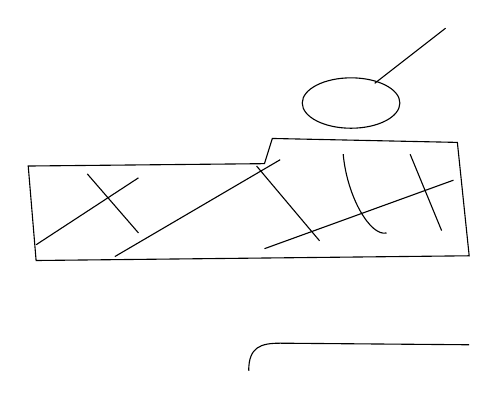
\begin{tikzpicture}[x=1cm,y=1cm]
\draw (4.1,3.7) ellipse (0.62 and 0.32); \draw (4.4,3.95)--(5.3,4.65);
\draw (0,2.9)--(0.1,1.7)--(5.6,1.76)--(5.45,3.2)--(3.1,3.25)--(3.0,2.93)--cycle;
\draw (0.1,1.9)--(1.4,2.75) (0.75,2.8)--(1.4,2.05) (1.1,1.75)--(3.2,2.98) (2.9,2.9)--(3.7,1.95) (3,1.85)--(5.4,2.72) (4,3.05)..controls (4.05,2.5) and (4.35,2)..(4.55,2.05) (4.85,3.05)--(5.25,2.08);
\draw (3.2,0.65)--(5.6,0.63); \draw (3.2,0.65)..controls (2.95,0.65) and (2.8,0.6)..(2.8,0.3);
\end{tikzpicture}}
\mspage{278}
